%!TEX root=finmath2.tex

\chapter{Модель Хестона: цены европейских опционов}
\label{ch:heston-formula}
\chaptertoc

Модель Хестона (S.~Heston, 1993) "--- это одна из популярных моделей стохастической волатильности.
Ее главное достоинство состоит в том, что в ней имеется формула для цен европейских опционов колл и пут, которая сводится к вычислению некоторого интеграла, что позволяет быстро находить цены опционов численно.

\section{Описание модели}
\subsection{Уравнения, задающие модель}

Далее всегда будем считать, что исходная вероятностная мера $\P$ уже является мартингальной.
Кроме того, для простоты изложений и краткости формул мы будем предполагать, что безрисковая процентная ставка нулевая, а рисковый акив не платит дивиденды (о том, как к такому случаю свести общую модель, см.~раздел \ref{gen:s:forward} лекции \ref{ch:general}).

Цена рискового актива в модели Хестона описывается уравнениями
\begin{align}
\label{hes:S}
&dS_t = \sqrt{V_t}S_t d W_t^{(1)},\\
\label{hes:V}
&d V_t = \kappa(\theta-V_t)dt + \xi\sqrt{V_t} d W_t^{(2)},
\end{align}
где процесс $V_t$ называется \emph{стохастической дисперсией} ($\sqrt{V_t}$ "--- \emph{стохастическая волатильность}), $W_t^{(1)},W_t^{(2)}$ "--- стандартные броуновские движения с коэффициентом корреляции $\rho\in(-1,1)$, \te\ $\E(W_t^{(1)}W_t^{(2)}) = \rho t$.
Величины $\kappa,\theta,\xi>0$, $\rho\in(-1,1)$, а также начальное значение $V_0\ge 0$ являются параметрами модели, которые нужно оценить из рыночных данных.
Отметим, что процесс стохастической дисперсии $V_t$ "--- это процесс CIR, рассмотренный в лекции \ref{ch:sde}.

Начальные условия $S_0$ и $V_0$ далее всегда будет считаться строго положительными.

\begin{proposition}
Система уравнений \eqref{hes:S}--\eqref{hes:V} имеет единственное сильное решение $(S,V)$, причем процесс $S_t$ строго положителен.
Двумерный процесс $(S_t,V_t)$ является строго марковским.
Если $2\kappa\theta\ge \xi^2$, то процесс $V_t$ строго положителен. 
\end{proposition}

\begin{proof}
Существование единственного сильного решения уравнения \eqref{hes:V}, а также то, что условие $2\kappa\theta\ge\xi^2$ (условие Феллера) приводит к положительности решения, обсуждалось в лекции \ref{ch:sde}.
Сильное решение уравнения \eqref{hes:S} можно построить в явном виде:
\[
S_t = S_0 e^{\int_0^t \sqrt{V_s} dW_s^{(1)}  - \frac12 \int_0^t V_s ds}.
\]
Проверка того, что это действительно решение проводится по формуле Ито.
Единственность (впрочем, как и существование) вытекает из того, что $S_t$ является \emph{стохастической экспонентой} процесса $d X_t = \sqrt{V_t} dW_t^{(1)}$ и общего результата о существовании и единственности стохастической экспоненты (см.~подробнее приложение \ref{ch:stoch-exp}).

Строго марковское свойство процесса $(S,V)$ следует из существования и единственности решения (см.~теорему \ref{sde:t:strong-markov} в лекции \ref{ch:sde}).
\end{proof}

Можно дать следующую интерпретацию параметрам процесса стохастической дисперсии.
Во-первых, заметим, что
\begin{equation}
\label{hes:EV}  
\E V_t = \theta + (V_0 - \theta)e^{-\kappa t}.
\end{equation}
Эта формула получается, если взять математическое ожидание от обеих частей интегральной формы уравнения \eqref{hes:V}.
Тогда, обозначая, $f(t) = \E V_t$, получаем уравнение $f(t) = V_0 + \kappa\int_0^t (\theta - f(s))ds$, решением которого является \eqref{hes:EV}.

Таким образом, процесс $V_t$ обладает свойством возврата к уровню $\theta$, называемому \emph{долгосрочным средним}.
Параметр $\kappa$ задает \emph{скорость возврата} к $\theta$.
Параметр $\xi$ называют \emph{волатильностью волатильности} (\emph{vol-of-vol}), он контролирует насколько сильны колебания волатильности.


\subsection{Мартингальность процесса цены \difficult}

Напомним (см.~лекцию \ref{ch:general}), что желательным свойством любой модели является настоящая (не локальная) мартингальность цены рискового актива $S_t$.

\begin{proposition}
\label{hes:p:price-martingale}
В модели Хестона процесс $S_t$ является мартингалом.
\end{proposition}

\begin{lemma}[\emph{теорема сравнения} для стохастических дифференциальных уравнений, см.~\cite{KaratzasShreve91}, гл.~5, предложение 2.18]
Пусть $X^{(1)}$ и $X^{(2)}$ "--- сильные решения уравнений
\[
d X_t^{(i)} = a^{(i)}(t, X_t^{(i)}) dt + b(t,X_t^{(i)}) d W_t, \qquad X_0^{(i)} = x_0^{(i)},
\]
заданные на одном вероятностном пространстве.
Предположим, что выполнены следующие условия:
\begin{enumerate}
\item функции $a^{(i)}(t,x)$, $b(t,x)$ непрерывны;
\item $|a^{(i)}(t,x) - a^{(i)}(t,y)| \le K|x-y|$ с некоторой константой $K>0$ для всех $t,x$ и хотя бы одного $i=1,2$;
\item найдется возрастающая функция $h(x)$ такая, что $h(0) = 0$, $\int_0^\epsilon h(x) dx = \infty$ для любого $\epsilon>0$, а также $|b(t,x) - b(t,y)| \le h(|x-y|)$ для всех $x,y$;
\item $x_0^{(1)} \le x_0^{(2)}$;
\item $b^{(1)}(t,x) \le b^{(2)}(t,x)$ для всех $t,x$;
\end{enumerate}
Тогда $X_t^{(1)} \le X_t^{(2)}$ \as\ для всех $t\ge 0$.
\end{lemma}

\begin{proof}[Доказательство предложения~\ref{hes:p:price-martingale}]
Как было отмечено выше, процесс $S_t$ является стохастической экспонентой процесса $d X_t = \sqrt{V_t}dW_t^{(1)}$.
Следовательно, для того, чтобы $S_t$ был мартингалом, достаточно выполнения условия Новикова (см.~приложение~\ref{ch:stoch-exp})
\[
\E \exp\biggl(\frac12 \int_0^T V_t dt\biggr) < \infty.
\]
В свою очередь, для этого достаточно (см.~следствие \ref{stochexp:novikov-corollary} в приложении \ref{ch:stoch-exp}), чтобы для некоторого $\epsilon>0$ и для всех $t\in[0, T-\epsilon]$ было выполнено неравенство
\[
\E \exp\biggl(\frac12 \int_t^{t+\epsilon} V_s ds\biggr) < \infty.
\]
Заметим, что по неравенству Йенсена $\exp(\int_t^{t+\epsilon} \frac 12 V_s ds) \le \frac1\epsilon\int_t^{t+\epsilon} \exp(\frac\epsilon2 V_s) ds$, а поэтому
\begin{equation}
\label{hes:mart-bound}
\E \exp\biggl(\frac12 \int_t^{t+\epsilon} V_s ds\biggr) 
\le \frac1\epsilon \int_t^{t+\epsilon} \E e^{\frac\epsilon2 V_s} ds.
\end{equation}
Оценим $\E e^{\frac\epsilon2 V_s}$.
Положим $n = 4\lceil \kappa\theta/\xi^2 \rceil$, $ \alpha = \kappa/2$ и рассмотрим процесс
\[
d V_t' = (n\xi^2/4 - 2\alpha V'_t) dt + \xi\sqrt{V_t'} d W_t^2, \qquad V_0' = V_0.
\]
Параметры $n$ и $\alpha$ выбраны так, что для всех $v\ge0$ выполнено неравенство $n\xi^2/4-2\alpha v \ge \kappa (\theta-v)$.
Тогда, используя теорему сравнения, находим, что 
\[
V_t' \ge V_t\ \text{\as\ для всех $t\ge 0$}.
\]

Таким образом, достаточно будет оценить сверху подходящим образом ожидание $\E e^{\frac\epsilon2 V_t'}$.
Для этого покажем, что верно равенство по распределению $V_t' \stackrel{d}{=} U_t$ для процесса
\[
U_t = \sum_{i=1}^n (Y_t^{(i)})^2,
\]
где $Y^{(i)}$ "--- независимые процессы Орнштейна"--~Уленбека
\[
d Y_t^{(i)} = -\alpha Y_t^{(i)} dt +  \frac\xi2 d B_t^{(i)}
\]
с начальными условиями $Y_0^{(i)}$ такими, что $\sum_i (Y_0^{(i)})^2 = V_0'$.

Действительно, применяя формулу Ито, получаем
\[
d U_t = \left(\frac{n\xi^2}{4}-2\alpha U_t\right) dt + \sum_{i=1}^n Y_t^{(i)} d B_t^{(i)} = 
\left(\frac{n\xi^2}{4}-2\alpha U_t\right) dt + \xi \sqrt{U_t} d Z_t
\]
с процессом 
\[
d Z_t = \frac{\sum_i Y_t^{(i)}}{\xi \sqrt{U_t}} d B_t^i.
\]
Процесс $Z_t$ является локальный мартингалом.
Кроме того, его квадратическая характеристика равна $t$ (\te\ $Z_t^t -t $ является локальным мартингалом), в чем нетрудно убедиться по формуле Ито, показав, что дифференциал $d(Z_t^2 - t)$ не содержит члена с $dt$.
Отсюда по теореме Леви%
\footnote{Непрерывный локальный мартингал с нулевым начальным значением является стандартным броуновским движением тогда и только тогда, когда его квадратическая характеристика равна $t$.}
следует, что $Z_t$ "--- стандартное броуновское движение и, значит, $U_t$ удовлетворяет тому же уравнению, что и $V_t'$, \te\ является процессом CIR с теми же параметрами.
Таким образом, $U$ и  $V'$  совпадают по распределению.

Так как процессы Орнштейна"--~Уленбека $Y_t^i$ имеют гауссовские распределения, то для любого $c>1$ и всех $t\in[0,T]$ найдется малое $\epsilon>0$ такое, что $\E e^{\frac\epsilon2 (Y_t^i)^2} < c$, и тогда
\[
\E e^{\frac\epsilon2 V_t'} \le c^n.
\]
Отсюда следует, что правая часть \eqref{hes:mart-bound} конечна, что нам и требовалось.
\end{proof}


\subsection{Условие для безарбитражности модели \difficult}

Выше мы предполагали, что исходная вероятностная мера $\P$ уже является мартингальной.
Если же относительно меры $\P$ процесс цены $S_t$ имеет произвольный коэффициент сноса, то вопрос о существовании эквивалентной мартингальной меры и выполнении свойства безарбитражности (NFLVR) становится деликатным и зависит от выполнения условия Феллера.
Для простоты изложения, ограничимся случаем постоянной безрисковой ставки $r$ и постоянного коэффициента сноса $\mu$.

\begin{proposition}[см.~\cite{DesmettreLeobacherRogers21}]
Пусть относительно меры $\P$ цена рискового актива задается уравнениями
\begin{align*}
&d S_t = \mu S_t dt + \sqrt{V_t} d W_t^{(1)},\\
&d V_t = \kappa(\theta-V_t)dt + \sigma \sqrt{V_t} d W_t^{(2)},
\end{align*}
где $\mu\neq r$.
Тогда ЭЛММ в такой модели существует в том и только том случае, когда выполнено условие Феллера $2\kappa\theta\ge \sigma^2$.
\end{proposition}


\section{Формула для цены европейских опционов}

В этом разделе будет получена формула для цен ванильных опционов колл и пут в модели Хестона, которая сводится к вычислению некоторого интеграла.
Значение этого интеграла можно найти методами численного интегрирования.

Идея будет состоять в том, чтобы сначала выразить цену опциона через вероятности его исполнения относительно двух вероятностных мер, затем получить аналитическую формулу для характеристических функций логарифма цены рискового актива относительно этих мер и, обратив их, найти вероятности исполнения опциона.
Упомянутый выше интеграл будет возникать при обращении характеристических функций.

Далее будем рассматривать только опционы колл.
Цены пут можно найти аналогично или воспользоваться паритетом цен колл-пут.


\subsection{Формулировка теоремы}

Зафиксируем время исполнения $T$. Определим функции
\begin{align*}
&\phi(u;t,x,v) = \exp(C(T-t,u) + D(T-t,u)v + iu x),& &u\in\R_+ \cup (\R_+-i),\\
&\tilde \phi(u;t,x,v) = e^{-x}\phi(u-i;t,x,v),& &u\in\R_+,
\end{align*}
где
\begin{align}
\label{hes:C}
&C(\tau,u) = \frac{\kappa\theta}{\sigma^2}
  \biggl(
    (\kappa- \rho\sigma iu - d(u))\tau 
    - 2\ln\biggl(\frac{1-g(u)e^{-d(u)\tau}}{1-g(u)}\biggr)
  \biggr),\\
\label{hes:D}
&D(\tau,u) = \frac{\kappa - \rho\sigma i u - d(u)}{\sigma^2}
  \biggl(\frac{1-e^{-d(u)\tau}}{1-g(u)e^{-d(u)\tau}}\biggr),\\
\label{hes:dg}
&d(u)=\sqrt{(\rho\sigma iu - \kappa)^2 + \sigma^2(iu + u^2)},\quad
  g(u) = \frac{\rho\sigma iu- \kappa +d(u)}{\rho\sigma iu - \kappa -d(u)}.
\end{align}
Здесь везде $i=\sqrt{-1}$ "--- мнимая единица. Множество $\R_+-i$ обозначает полупрямую в комплексной плоскости, параллельную неотрицательной действительной полуоси и исходящую из точки $-i$.
Переменные $t,x,v$ вещественные.

Как будет видно далее, $\phi$ является условной характеристической функцией $\E (e^{iu X_T}\mid X_t=x, V_t=v)$, где $X_t=\ln S_t$, а $\tilde \phi$ "--- это та же характеристическая функция, но вычисленная по другой мере.

В следующей теореме, как и прежде, считается, что безрисковая процентная ставка равна нулю, а базовый актив не выплачивает дивиденды.

\begin{theorem}[С.~Хестон]
\label{hes:t:formula}
Цена опциона колл со страйком $K$ и временем исполнения $T$ в момент времени $t$ равна
\begin{equation}
\label{hes:call-repr}
C_t = C(t,\ln S_t,V_t),
\end{equation}
где функция $C$ имеет вид
\begin{equation}
\label{hes:call-undiscounted}
C(t,x,v) = e^x \tilde \Pi(t,x,v) - K \Pi(t,x,v)
\end{equation}
с функциями $\tilde\Pi$, $\Pi$ определенными по формулам
\begin{align}
\label{hes:pi}
&\Pi(t,x,v) = \frac12 + \frac1\pi \int_0^\infty
  \mathrm{Re}\biggl(\frac{e^{-iu \ln K}\phi(t,x,v;u)}{iu}\biggr) du,\\[0.5em]
\label{hes:pit}
&\tilde\Pi(t,x,v) = \frac12 + \frac1\pi \int_0^\infty
  \mathrm{Re}\biggl(\frac{e^{-iu \ln K}\tilde \phi(t,x,v;u)}{iu}\biggr) du.
\end{align}
\end{theorem}

\begin{remark}
В формулах \eqref{hes:C} и \eqref{hes:dg} присутствуют комплексный корень и комплексный логарифм, являющиеся, вообще говоря, многозначными функциями.
Несмотря на то, что утверждение теоремы справедливо при любом выборе ветвей этих функций, удобнее всего здесь взять их главные значения%
\footnote{Напомним, что для числа $z\in\mathbb{C}$, записанного в виде $z=re^{i\phi}$, $r\ge 0$, $\phi\in(-\pi,\pi]$, главные значения логарифма и квадратного корня определены как $\ln z = \ln r + i\phi$ и $\sqrt{z} = \sqrt{r}e^{i\phi/2}$ (логарифм не определен для $z=0$).}. Это обеспечит непрерывность функций $C$ и $D$ на множестве $u\in\R_+$ и $u\in (\R_+-i)$, что положительно сказывается на работе методов численного интегрирования для нахождения $\Pi$ и $\tilde\Pi$.

Доказательство непрерывности технически нетрудное, но достаточно громоздкое, см.~детали в статье \cite{Albrecher+05}.
Основная его идея состоит в том, что когда $u$ пробегает множество $\R_+$ или $\R_+-i$, аргументы логарифма и корня не пересекают отрицательную действительную полуось, что влечет их непрерывность в силу использования главных ветвей.
\end{remark}


\subsection{Доказательство}
\subsubsection{Представление цены опциона через вероятности исполнения}

Первый шаг будет состоять в том, чтобы выразить цену опциона колл через вероятности его исполнения по двум мерам.
Отметим, что приводимая ниже лемма выполнена не только в модели Хестона, но вообще в любой безарбитражной модели, при условии что безрисковая ставка равна 0, рисковый актив не выплачивает дивиденды, а его цена является настоящим мартингалом относительно меры $\P$.

Зафиксируем момент исполнения $T$ и определим новую вероятностную меру $\tilde\P$ с плотностью
\[
\frac{d\tilde\P}{d\P} = \frac{S_T}{S_0}. 
\]

\begin{lemma}
\label{hes:l:price-through-prob}
Цена опциона колл со страйком $K$ и временем исполнения $T$ в момент $t$ представима в виде 
\[
C_t = S_t \tilde\P(S_T\ge K\mid \F_t) - K\P(S_T\ge K\mid \F_t).
\]
\end{lemma}

\begin{proof}
Заметим, что
\[
C_t = \E^\P((S_T - K)^+\mid \F_t) = \E^\P(S_T \I(S_T\ge K) \mid \F_t) - K\P(S_T\ge K\mid \F_t).
\]
Пусть $Z = S_T/S_0$ обозначает плотность $d\tilde\P/d\P$. 
Тогда из формулы пересчета для условных математических ожиданий (см.~замечание ниже) находим
\begin{multline*}
\tilde\P(S_T\ge K\mid \F_t) = \E^{\tilde\P} (\I(S_T \ge K) \mid \F_t)
= \frac{\E^{\P}(Z \I(S_T \ge K)\mid \F_t)}{\E^{\P}(Z\mid \F_t)} \\= S_t \E^{\P}(S_T \I(S_T\ge K)\mid \F_t),
\end{multline*}
где воспользовались тем, что $\E(Z\mid \F_t) = S_t/S_0$, так как $S_t$ "--- мартингал относительно меры $\P$.
Подставляя получившееся равенство в формулу выше, получаем доказываемое утверждение.
\end{proof}

\begin{remark}
\emph{Формула пересчета} для условных математических ожиданий утверждает, что для двух мер $\tilde\P \sim \P$ с плотностью $Z=d\tilde\P/d\P$, произвольной $\sigma$-алгебры $\G\subseteq\F$ и $\tilde\P$-интегрируемой случайной величины $\xi$ верно равенство (см.~\cite{Shiryaev04}, гл.~II, \S\,7, теорема 6)
\[
\E^{\tilde \P}(\xi\mid \G) = \frac{\E^{\P}(Z\xi\mid \G)}{\E^\P(Z\mid \G)}.
\]
\end{remark}


\subsubsection{Характеристчиеские функции логарифма цены}

Будем работать с процессом логарифма цены рискового актива
\[
X_t = \ln S_t.
\]
Для $t\le T$ определим условные характеристические функции
\begin{align*}
&\phi(u; t,x,v) = \E^{\P} (e^{iu X_T} \mid X_t=x, V_t = v), \qquad u\in\R_+ \cup (\R_+-i),\\
&\tilde\phi(u; t,x,v) = \E^{\tilde\P} (e^{iu X_T} \mid X_t=x, V_t = v), \qquad u\in\R_+ .
\end{align*}
Второй шаг в доказательстве теоремы \ref{hes:t:formula} "--- вычисление функций $\phi$ и $\tilde\phi$.
Для начала покажем, что вычисление $\tilde\phi$ можно свести к $\phi$.

\begin{lemma}
Справедливо равенство $\tilde \phi(u; t,x,v) = e^{-x}\phi(u-i;t,v,x)$.
\end{lemma}

\begin{proof}
Имеем
\[
\begin{split}
\tilde\phi(u; t,x,v) &= \E^{\tilde\P} (e^{iu X_T}  \mid X_t=x, V_t = v)
= \frac{\E^{\P} (Z e^{iu X_T} \mid X_t=x, V_t = v)}{\E^\P(Z \mid X_t=x,V_t=v)} \\
&= e^{-x} \E^{\P} (e^{i(u-i)X_T} \mid X_t=x, V_t = v)
= e^{-x}\phi(u-i; t,x,v),
\end{split}
\]
где воспользовались формулой пересчета для условных ожиданий, а также тем, что $Z=S_T/S_0$ и $\E^\P(S_T  \mid X_t=x, V_t = v) = e^x$, так как $S_t$ "--- мартингал.
\end{proof}

\begin{lemma}
Для любого $u\in \R$ функция $\phi(u;t,x,v)$ является единственным решением задачи Коши (в классе $C^{1,2}$ на $[0,T)\times\R\times\R_+$)
\begin{align}
\label{hes:cf-pde}
&\frac{\partial\phi}{\partial t} + \frac v2 \frac{\partial^2 \phi}{\partial x^2}  +\frac{\sigma^2v}{2} \frac{\partial^2\phi}{\partial v^2}
  + \rho\sigma v \frac{\partial^2\phi}{\partial x\partial v} -\frac v2 \frac{\partial \phi}{\partial x} 
  + \kappa(\theta-  v)\frac{\partial\phi}{\partial v} = 0,\\
\label{hes:cf-boundary}
&\phi(u;T,x,v) = e^{iu x}.
\end{align}
\end{lemma}

\begin{proof}
Этот результат напрямую следует из формулы \fc\ (см.~лекцию \ref{ch:sde}), применяя ее к вещественной и мнимой частям $\phi$.
\end{proof}

Покажем теперь, как решить задачу Коши \eqref{hes:cf-pde}--\eqref{hes:cf-boundary}.
Идея состоит в том, чтобы искать решение в специальном виде
\begin{equation}
\label{hes:cf}
\phi(u; t,x,v) = \exp(C(T-t,u) + D(T-t,u)v + iu x)
\end{equation}
с неизвестными функциями $C(\tau,u)$ и $D(\tau,u)$.
Чтобы их найти, подставим $\phi$ такого вида в \eqref{hes:cf-pde} и получим уравнение
\begin{equation}
\label{hes:CD-equation}
v\biggl(
  -\prt{D}\tau + \rho\sigma iu D - \frac12 u^2 
  + \frac12 \sigma^2 D^2 -\frac12 iu-\kappa D
\biggr) + \biggl(-\prt{C}\tau + \kappa\theta D\biggr) = 0.
\end{equation}
Равенство будет выполнено, если каждая из скобок тождественно равна нулю.
Заметим, что первая скобка не содержит функцию $C$, что приводит к обыкновенному дифференциальному уравнению на функцию $D$:
\[
D' = \rho\sigma ui D + \frac12 (\sigma^2 D^2 - iu - u^2) - \kappa D, \qquad D(0,u)=0,
\]
где штрих обозначает производную по переменной $\tau$, а переменная $u$ является фиксированным параметром.
Начальное условие $D(0,u)=0$ возникает из того, что $\phi(u,T,x,v) = \exp(iux)$ по определению функции $\phi$, а тогда из формулы \eqref{hes:cf} видно, что значение $D(0,u)$ должно быть равно 0 для всех $u$.

Уравнение для $D$ является \emph{уравнением Риккати} и решается известными методами.
Для удобства запишем его в виде
\[
D'= \alpha + \beta D + \gamma D^2,
\]
где
\[
\alpha = -\frac{iu + u^2}{2},\qquad \beta = \rho\sigma iu - \kappa, \qquad
\gamma = \frac{\sigma^2}{2}.
\]
Нетрудно проверить, что если функция $z(\tau)$ является решением уравнения
\[
z''(\tau) - \beta z(\tau) + \alpha\gamma z(\tau)= 0,
\]
то
\[
D(\tau,u) = -\frac{z'(\tau)}{\gamma z(\tau)} 
\]
является решением исходного уравнения.

Уравнение для $z(\tau)$ линейное, и хорошо известно его общее решение.
Для этого рассмотрим характеристическое уравнение $r^2-\beta r+\alpha\gamma = 0$.
Непосредственно проверяется, что при любых значениях параметров модели Хестона и $u\in\R_+$ или $u\in(\R_+-i)$ дискриминант $d = \sqrt{(\rho\sigma iu - \kappa)^2 + \sigma^2(iu + u^2)}$ не обращается в нуль и, следовательно, общее решение имеет вид
\[
z(\tau) = K_1 e^{r_1\tau} + K_2 e^{r_2\tau},
\]
где $K_1,K_2$ "--- свободные константы, а $r_1=(\beta+d)/2$ $r_2=(\beta-d)/2$ "--- корни характеристического уравнения.
Это дает
\[
D(\tau) = -\frac1\gamma \biggl(\frac{K_1 r_1 e^{r_1\tau} + K_2 r_2e^{r_2\tau}}{K_1 e^{r_1\tau} + K_2e^{r_2\tau}} \biggr),
\]
Чтобы получить решение, удовлетворяющее начальному условию $D(0,u)=0$, выберем
\[
K_1 = 1, \qquad K_2 = -\frac{r_1}{r_2},
\]
что после преобразований приводит к формуле \eqref{hes:D} для $D(\tau, u)$.

Затем функцию $C$ нетрудно найти из условия равенства нулю второй скобки в уравнении \eqref{hes:CD-equation} и начального условия $C(0,u)=0$ (возникающего по той же причине, что и для $D$).
Получаем
\[
C(\tau, u) = \kappa\theta \int_0^\tau D(s,u) ds.
\]
Вычисляя интеграл, приходим к формуле \eqref{hes:C}.
Подытоживая приведенные рассуждения, получаем следующий результат.

\begin{lemma}
Решением задачи \eqref{hes:cf-pde}--\eqref{hes:cf-boundary} является функция $\phi$ вида \eqref{hes:cf}, в которой $D(\tau,u)$ и $C(\tau,u)$ заданы по формулам \eqref{hes:C}--\eqref{hes:dg}.
\end{lemma}


\subsubsection{Обращение характеристических функций и завершение доказательства}

\begin{lemma}[\emph{формула обращения}, см.~\cite{GilPelaez51}] 
Пусть $\phi(u)$ "--- характеристическая функция распределения $F(x)$, \te\ $\phi(u) = \int_\R e^{iu x} d F(x)$.
Тогда
\[
F(x) = \frac 12 - \frac1\pi 
\int_0^\infty \mathrm{Re}\biggl(\frac{e^{-iu x}\phi(u )}{iu}\biggr) d u.
\]
\end{lemma}

Обозначим теперь $\Pi(t,x,v)$ и $\tilde\Pi(t,x,v)$ условные вероятности исполнения опционов:
\begin{align*}
&\Pi(t,x,v) = \P(\ln X_T \ge \ln K \mid X_t =x , V_t=v), \\
&\tilde \Pi(t,x,v) = \tilde \P(\ln X_T \ge \ln K \mid X_t =x , V_t=v)
\end{align*}
Тогда по формуле обращения получаем для $\Pi$ и $\tilde\Pi$ представления \eqref{hes:pi}--\eqref{hes:pit}.

Остается воспользоваться тем, что $(S_t,V_t)$ и, следовательно $(X_t,V_t)$, являются марковскими процессами, а поэтому в лемме \eqref{hes:l:price-through-prob} можно заменить вероятность $\P(S_T\ge K\mid \F_t)$ на $\Pi(t, X_t, V_t)$ (и, аналогично, $\tilde \P(S_T\ge K\mid \F_t)$), что даст доказываемую формулу для цены опциона.


\section{Калибровка модели. Качественная роль параметров}

Под \emph{калибровкой модели} понимается задача определения ее параметров (например, для модели Хестона это набор $\Theta=(V_0,\kappa,\theta,\sigma,\rho)$).
Для базовых активов, у которых имеется ликвидный рынок ванильных опционов, стандартным способом калибровки является минимизация статической ошибки, \te\ ставится цель найти параметры, при которых модель дает цены опционов наиболее близкие к рыночным.

При этом, обычно сравнивают не сами цены опционов, а их подразумеваемые волатильности%
\footnote{По той причине, что подразумеваемые волатильности для разных опционов являются величинами <<одного порядка>>, а цены опционов могут весьма сильно различаться.}.
А именно, пусть $\hat\sigma_\text{model}(T,K; \Theta)$ обозначает подразумеваемую волатильность опциона с временем исполнения $T$ и страйком $K$ в модели с набором параметров $\Theta$, а $\hat\sigma_\text{market}(T,K)$ обозначает рыночную подразумеваемую волатильность.
Пусть рыночные волатильности даны для пар $(T_i,K_i)_{i=1}^n$.
Тогда решается задача 
\begin{equation}
\label{hes:calibration}
\sum_{i=1}^n (\hat\sigma_\text{model}(T_i,K_i;\Theta) - \hat\sigma_\text{market}(T_i,K_i))^2 \xrightarrow[\Theta]{} \min.
\end{equation}
Параметры $\Theta$, на которых достигается минимум, находятся численно. 

После того, как модель откалибрована, ее можно использовать для нахождения цен и хеджирования других производных инструментов.
Более детально мы обсудим эти вопросы в следующей лекции.

\begin{remark}
Говоря подробнее о задаче \eqref{hes:calibration}, величины $\hat\sigma_\text{model}$ вычисляются следующим образом.
Пусть безрисковая процентная ставка $r_t$ не обязательно нулевая (но детерминированная), а рисковый актив может выплачивать дивиденды непрерывным образом со ставкой доходности $q_t$. 
Модель изменения безрисковой ставки и дивидендной доходности нам здесь не важна, но будем считать, что известны цены бескупонных облигаций $B(0,T_i)$ (их нужно вычислить из рыночных данных, см.~подробнее лекцию 12 в курсе \intro).

Как следует из предложения \ref{gen:c:forward-vol} в лекции \ref{ch:general}, считая, что исходная вероятностная мера уже является мартингальной, в модели Хестона $T$-форвардная цена удовлетворяет уравнению
\begin{align*}
&dF_t^T = \sqrt{V_t}F_t^T dW_t^{(1)},\\
&dV_t = \kappa(\theta-V_t)dt + \sigma\sqrt{V_t} dW_t^{(2)},
\end{align*}
где начальное значение $F_0^{T}$ можно найти, например, из улыбки волатильности для срока исполнения $T$ через паритет цен колл-пут.
Тогда для нахождения подразумеваемой волатильности нужно вычислить цены опционов колл или пут
\[
\VC_i= B(0,T_i)\E (F_{T_i}^{T_i} - K)^+ 
\qquad(\text{или}\ \VP_i= B(0,T_i)\E (K-F_{T_i}^{T_i})^+),
\]
а затем найти $\hat\sigma_\text{model}(T_i,K_i;\Theta)$, обратив формулу Блэка.
\end{remark}

В заключение покажем, как параметры модели влияют на форму улыбок волатильности.
Для этого рассмотрим исходную модель с начальной ценой $S_0=1$ и параметрами
\[
V_0=0.09, \quad \kappa=2, \quad \theta=0.09,\quad  \sigma=1, \quad \rho=-0.5
\]
и посмотрим, как будут изменяться улыбки волатильности для времен исполнения $T=0.5$ и $T=2$ при изменении одного из параметров модели.
Результаты представлены на рис.~\ref{hes:f:smiles}.
Из него качественно можно сделать следующие выводы.
\begin{itemize}
\item Параметры $V_0$ и $\theta$, главным образом, отвечают за вертикальное положение улыбок волатильности, причем  $V_0$ больше влияет на улыбки с близким сроком исполнения, а $\theta$ "--- с дальним.
При увеличении этих параметров улыбки смещаются вверх.
\item Параметры $\kappa$ и $\xi$, главным образом,  отвечает за выпуклость улыбок.
При увеличении $\kappa$ улыбки становятся более выпуклыми, а при увеличении $\xi$ более плоскими.
\item Параметр $\rho$, главным образом, отвечает за наклон улыбок. Чем меньше его значение, тем более крутой левый хвост имеет улыбка. 
\end{itemize}

\begin{figure}[h]
\centering
  \begin{subfigure}{0.8\textwidth}
    \centering
    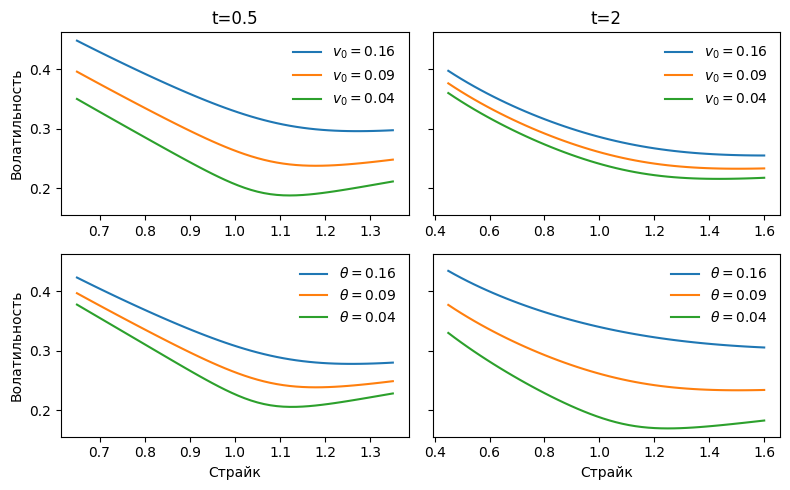
\includegraphics[width=12cm]{pic/heston-v0-theta.png}
    \caption{$V_0$ и $\theta$ влияют на вертикальное положение.}
    \label{hes:f:v0-theta}
  \end{subfigure}
  \begin{subfigure}{0.8\textwidth}
    \centering
    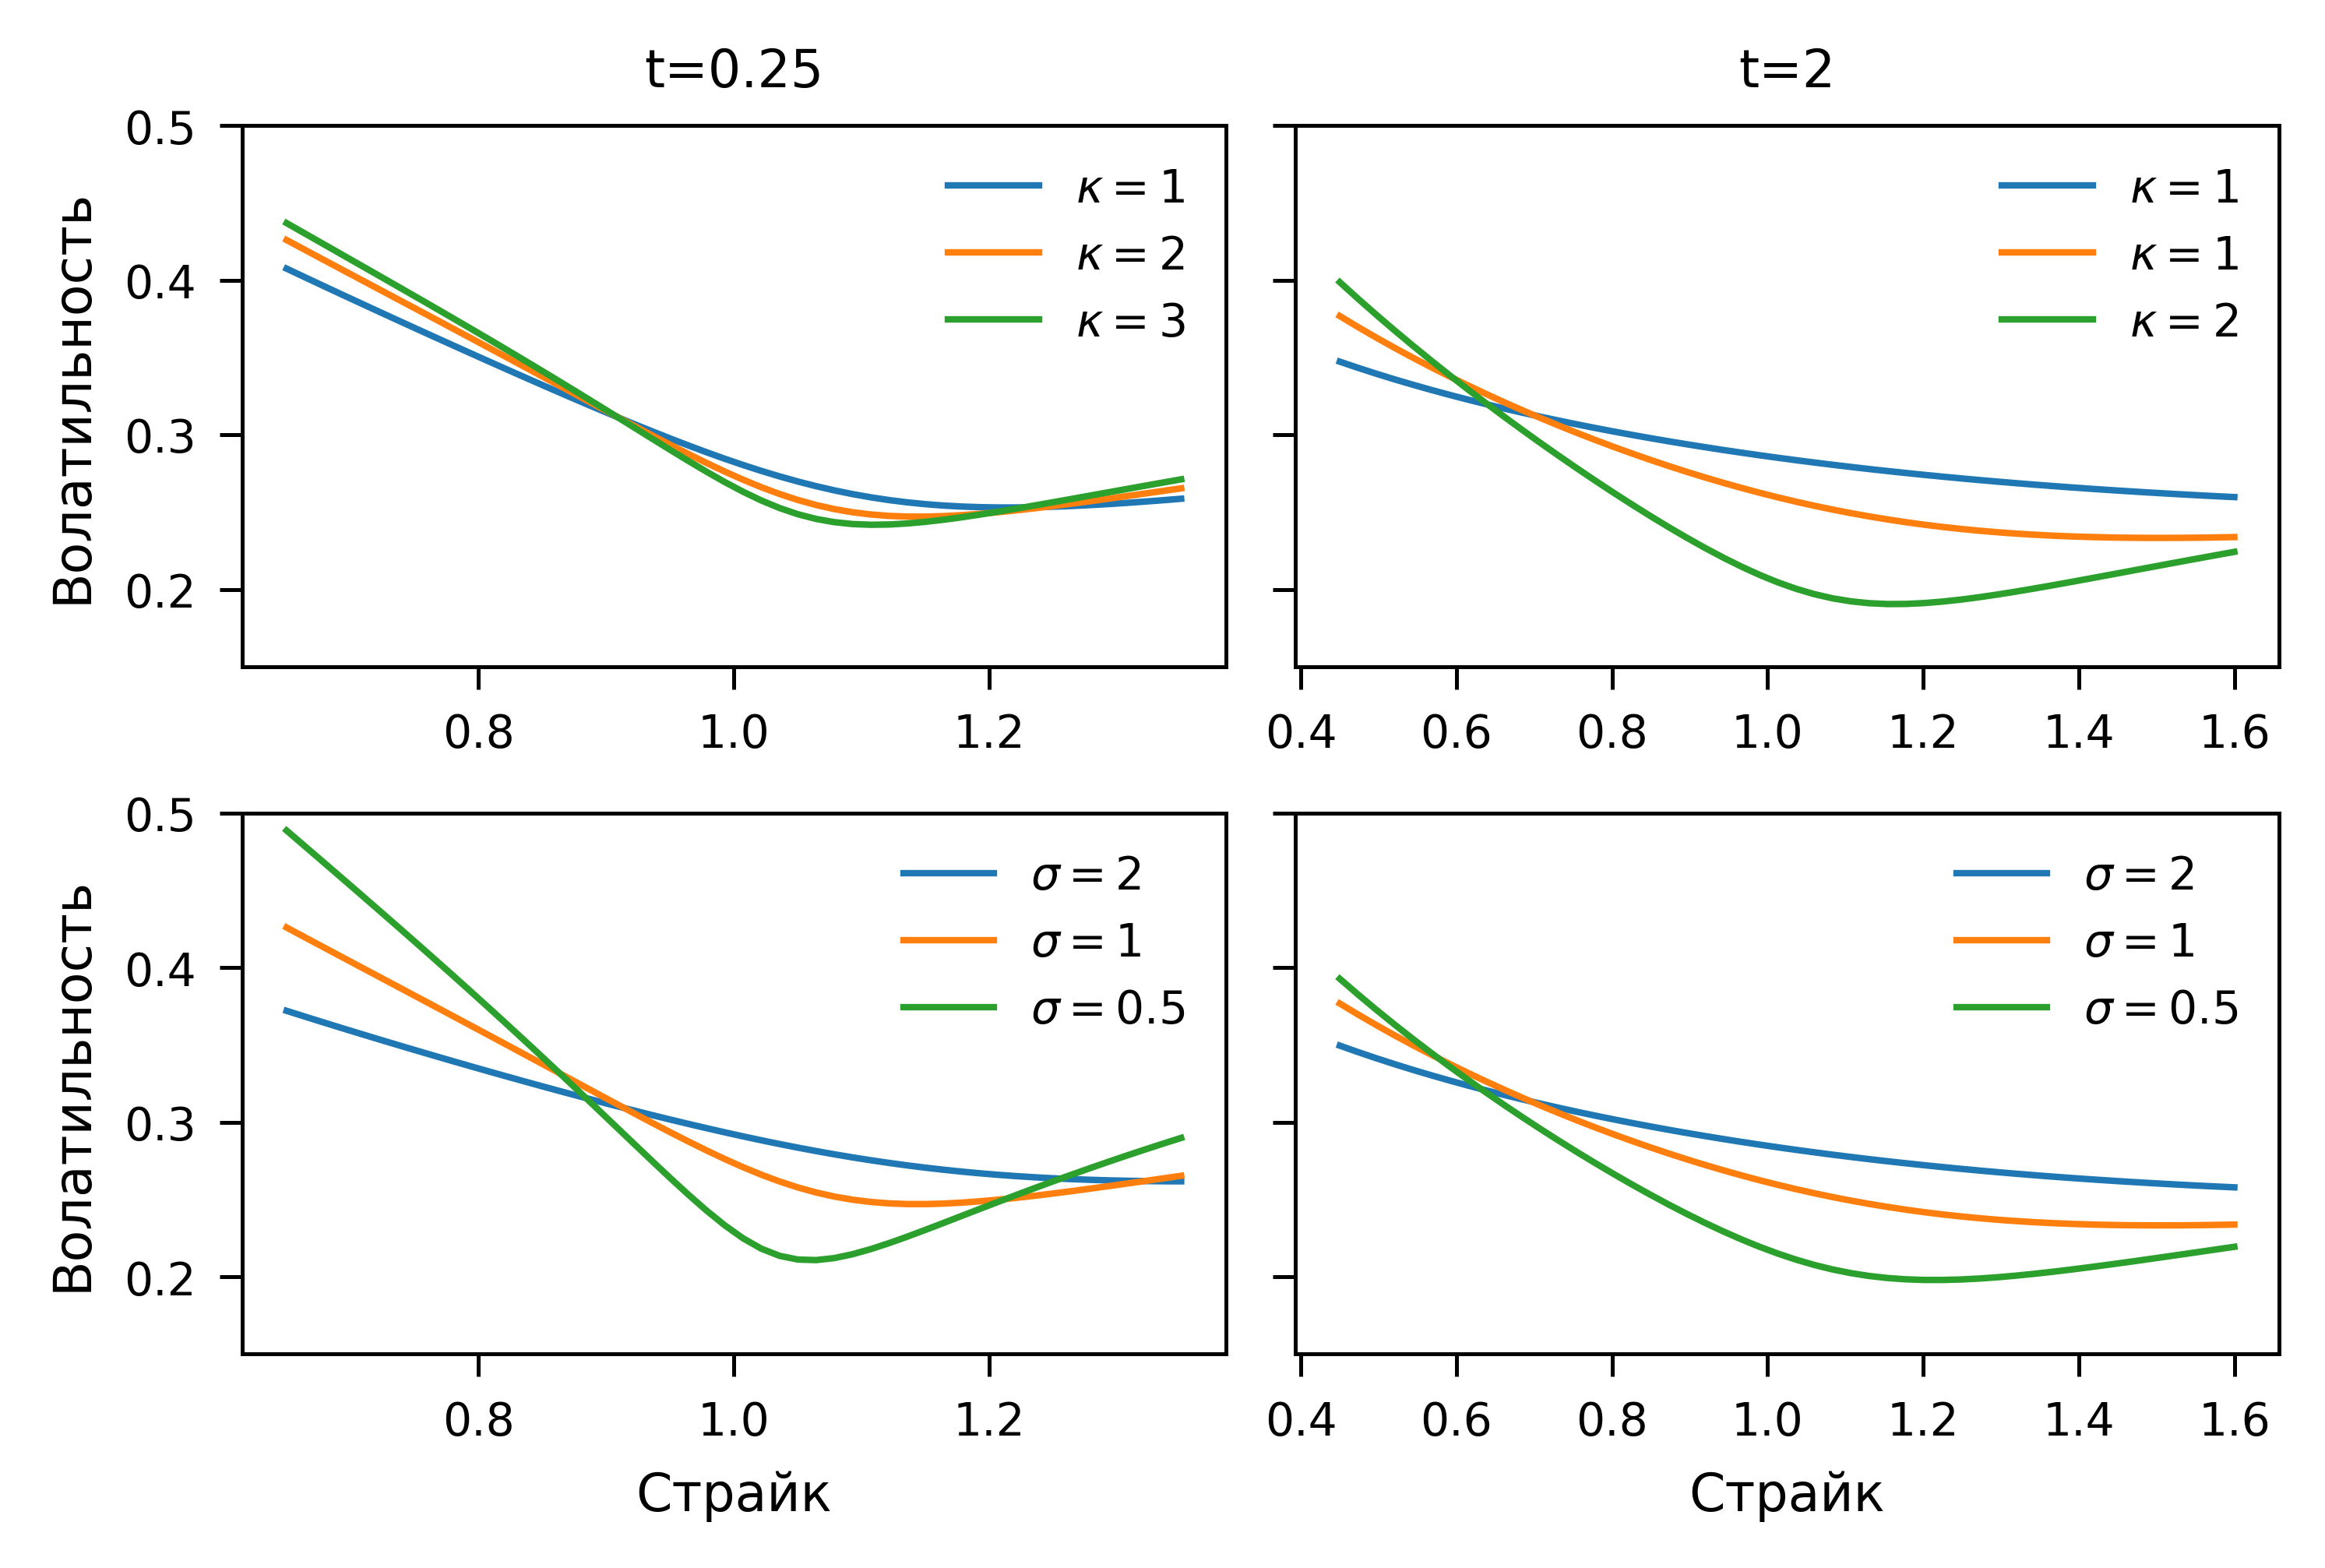
\includegraphics[width=12cm]{pic/heston-kappa-sigma.png}
    \caption{$\kappa$ и $\sigma$ влияют на выпуклость.}
    \label{hes:f:kappa-sigma}
  \end{subfigure}
  \begin{subfigure}{0.8\textwidth}
    \centering
    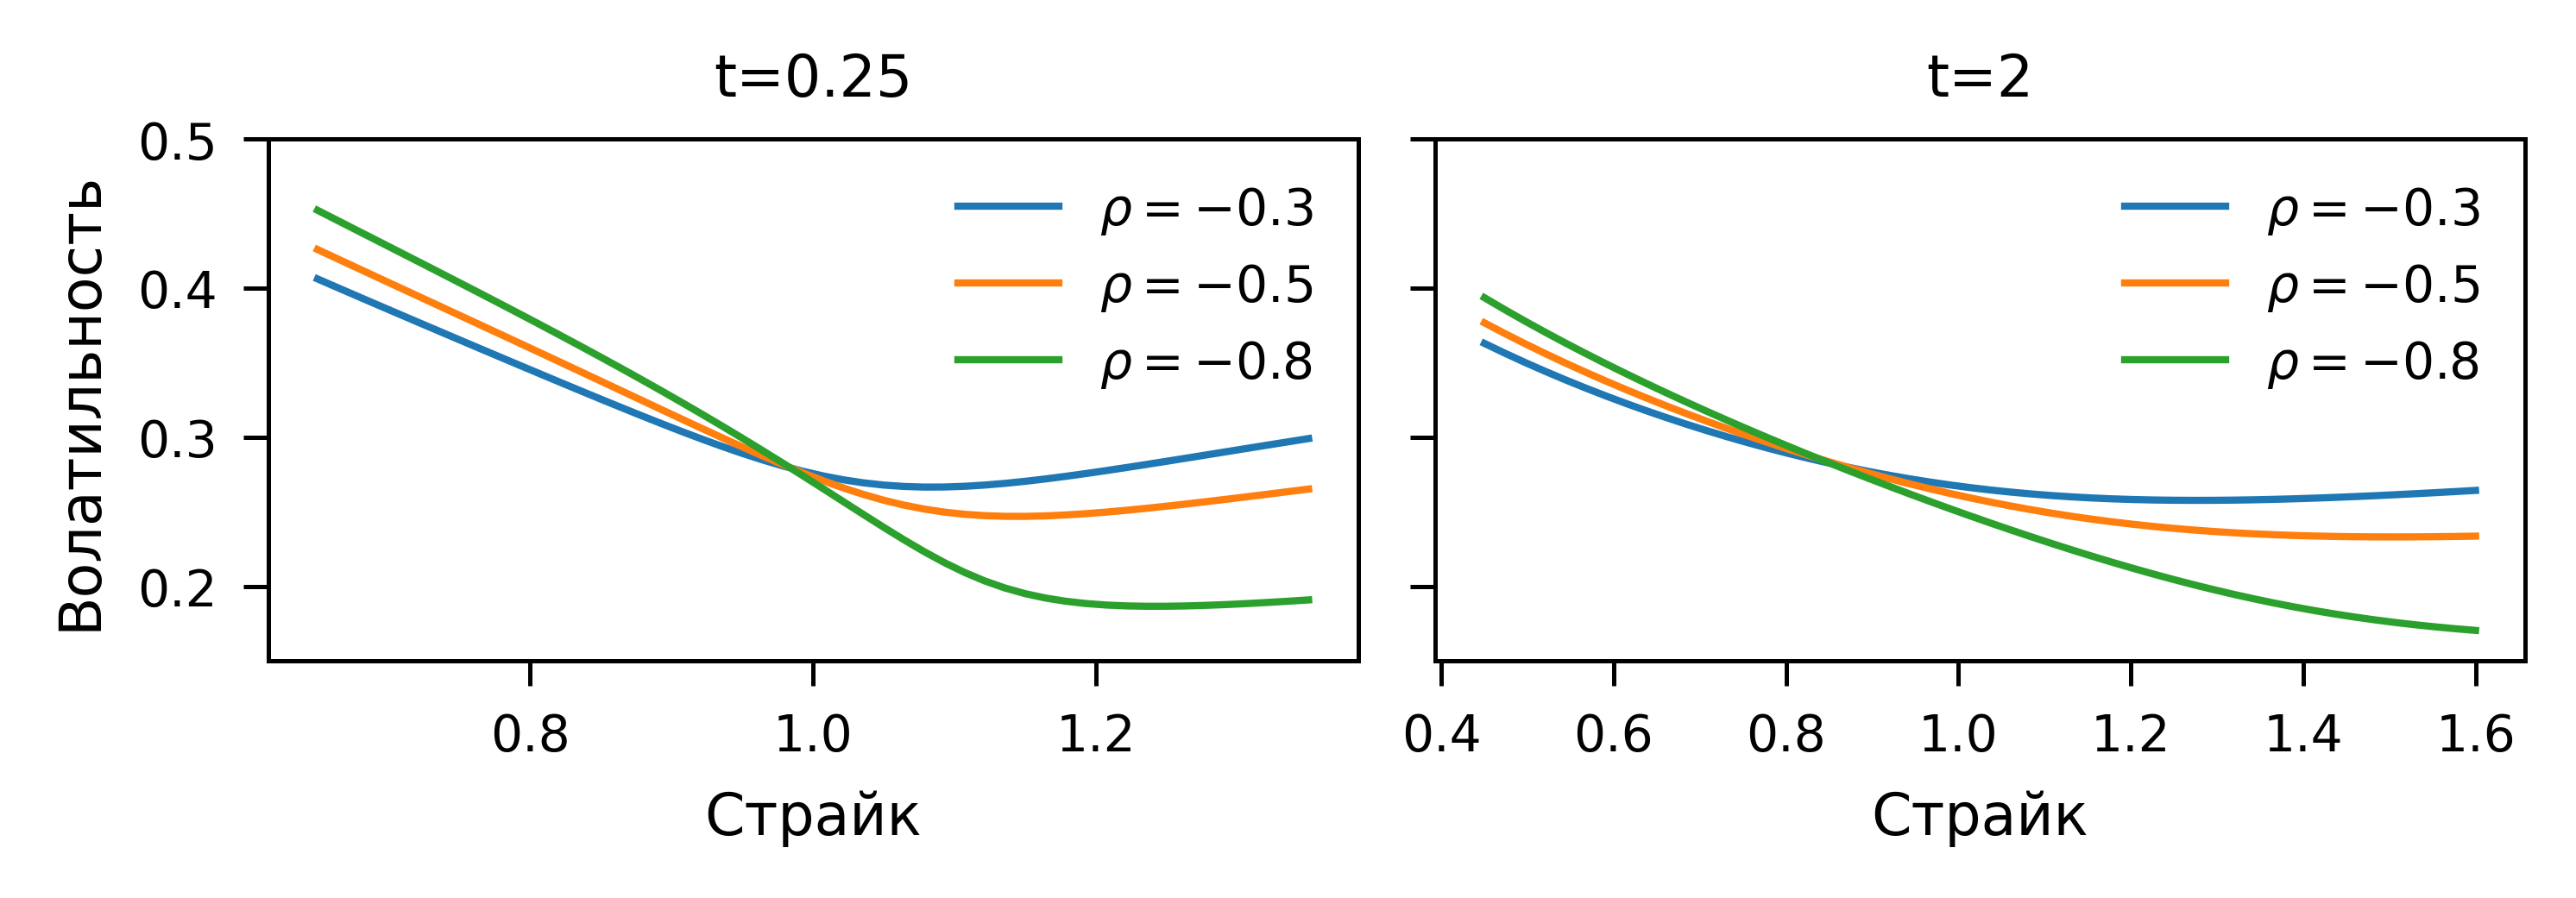
\includegraphics[width=12cm]{pic/heston-rho.png}
    \caption{$\rho$ влияет на наклон.}
    \label{hes:f:rho}
  \end{subfigure}
\caption{Влияние параметров модели Хестона на улыбки волатильности.}
\label{hes:f:smiles}
\end{figure}
